% !Mode:: "TeX:UTF-8"
\documentclass[type=doctor, openany, pifootnote]{shuthesis}
% 选项:
%  type=[master|doctor],            % 必选
%  secret,                          % 可选 (如果论文需要保密, 这一项需要打开)
%  pifootnote,                      % 可选(建议打开)
%  openany|openright,               % 可选 (章首页是右开还是任意开, 默认是右开)
%  nocolor                          % 提交最终版本时请打开此选项
\usepackage{pdfpages}
\usepackage{shuthesis}
\usepackage{times}

\graphicspath{{figures/}}

%\setCJKmainfont{FandolSong-Regular}[BoldFont=FandolHei-Regular,ItalicFont=FandolKai-Regular] % Linux
%\setCJKmainfont{Songti SC Light}[BoldFont=Heiti SC Light,ItalicFont=Kaiti SC, BoldItalicFont=Kaiti SC Bold] % MacOS 
\begin{document}

\includepdf[pages={1}]{cover.pdf} 

\frontmatter
{
    \hypersetup{linkcolor=black}
    \tableofcontents
}
\newpage

{
    % \cleardoublepage% Move to first page of new chapter
    \let\clearpage\relax% Don't allow page break
    \centering\zihao{1}{\textbf{基于机器学习的子宫肉瘤患者的临床病理及预后分析}}

    \vspace{8mm}

    \chapter*{摘\ 要}
}
\addcontentsline{toc}{chapter}{摘\ 要}

子宫肉瘤是源于子宫体部位的一组独立的高度恶性肿瘤,根据原发部位又分为子宫平滑肌肉瘤、子宫内膜间质肉瘤等。该肿瘤属于较为罕见的肿瘤,通常发病于45岁以上的绝经后妇女,虽然已经有一些相关文献对其进行了科普与介绍,关于其临床病理及预后分析的研究依然较少。本文基于SEER癌症数据集使用KM曲线与Cox多因素比例风险回归模型对影响其患者生存率的各个因素进行了分析与总结;并根据其预后相关数据进行了多种聚类算法的使用,分析聚类后得到簇所代表的表型具有的特征,从而分析得到子宫肉瘤患者的不同表型特点。由于聚类算法属于无监督学习,难以运用在新的数据上。所以本文建立了相关预后模型,使用决策树与随机森林对SEER上的聚类得到的表型进行训练,从而得到能区分患者所对应表型的预后模型,从而更好地评估患者的生存情况。最后结合医院提供的数据对上述模型进行了验证,总结全文工作与创新点,并展望后续工作。

\vspace{8mm}
\textbf{关键词}: 机器学习, 比例风险回归模型, 决策树, 随机森林, 层次聚类

\newpage
{
    % \cleardoublepage% Move to first page of new chapter
    \let\clearpage\relax% Don't allow page break
    \centering\zihao{1}{Machine learning-based clinicopathological and prognostic analysis of patients with uterine sarcoma}
    \vspace{8mm}

    \chapter*{ABSTRACT}
}
\addcontentsline{toc}{chapter}{ABSTRACT}

Uterine sarcoma is an independent group of highly malignant tumors originating from the body of the uterus, which are classified into smooth muscle sarcoma and endometrial mesenchymal sarcoma according to the site of origin. It is a rare tumor that usually develops in postmenopausal women over 45 years of age. Although it has been popularized and introduced in the literature, there are still few studies on its clinicopathological and prognostic analysis. In this paper, we analyzed and summarized the factors affecting the survival rate of patients based on the SEER cancer dataset using the KM curve and Cox multifactor proportional risk regression model; and used various clustering algorithms to analyze the characteristics of the phenotypes represented by clusters after clustering to analyze the different phenotypic characteristics of patients with uterine sarcoma based on their prognosis-related data. Since clustering algorithms are unsupervised learning, they are difficult to apply on new data. Therefore, in this paper, a relevant prognostic model is developed and the phenotypes obtained from clustering on SEER are trained using decision trees and random forests to obtain a prognostic model that can distinguish the phenotypes corresponding to the patients and thus better assess the survival of the patients. Finally, the above models were validated with the data provided by the hospital, summarizing the full work and innovations and looking forward to the follow-up work.

\vspace{8mm}

\textbf{Keywords}: Machine learning, proportional risk regression models, decision trees, random forests, hierarchical clustering

\mainmatter
% !Mode:: "TeX:UTF-8"
\chapter{绪论}
\label{cha:intro}

本章主要介绍了子宫肉瘤研究的相关研究的研究背景及意义,分析了相关课题的研究方法与现状,最后列举了本文的研究目标内容与结构。

\section{研究背景与意义}

作为一种较为罕见的肿瘤,子宫肉瘤相关死亡率在子宫恶性肿瘤中中的比例在16\%以上\cite{commonView},目前的主要治疗方式是以手术为主,手术后一般会通过化疗(少数情况使用放疗)辅助,以确保最后效果。根据SEER数据分析显示,子宫肉瘤患者的中位年龄在65岁左右,发病原因有很多,根据对文献中的数据显示,子宫肉瘤可能与某些遗传基因的突变有关。而子宫肉瘤的复发情况较为常见。子宫肉瘤的复发是指在手术和治疗完成后术后阶段肿瘤重新生长并再次出现的一系列过程。子宫肉瘤的复发并不局限于原发病灶,也可能出现在周边组织内,包括子宫、输卵管、卵巢等等。按照文献显示,\uppercase\expandafter{\romannumeral1}、\uppercase\expandafter{\romannumeral2}期患者5年生存率为59\%,而\uppercase\expandafter{\romannumeral3}期则为22\%,\uppercase\expandafter{\romannumeral4}期为9\%。\cite{commonView}从数据中可以看出,子宫肉瘤预后结果中,复发的概率较高,预后的效果较差。在预防子宫肉瘤的复发中,一些研究表明了术后辅助治疗和放疗能够达到降低复发率的作用,并提高患者的生存率。然而作为一种较少见的恶性肿瘤,目前子宫肉瘤方面尚未有比较公认的预后处理模型出现。为了处理近年各个医院积累的子宫肉瘤的随访与预后数据,利用数据对患者术后复发状况或生存率进行预测与评估,能够更好地帮助患者了解自身身体状况,也能帮助医生对于危险程度较高的患者进行重点关注,从而能够让医疗资源能够更加有效地被利用。因此,本文旨在建立一套使用患者预后数据训练而成的预后模型,并建立相应的UI界面,让医学人士能够方便地管理并使用该系统对于患者的将来的生存状况进行评估。

\section{子宫肉瘤研究发展现状}

目前,子宫肉瘤的研究尚且不是很多,有很多种ML模型可以在其中子宫肉瘤的检测分析中起到一定作用,比较常用的模型主要分为以下两类:图像模型、数据模型。

\subsection{在子宫肉瘤方面使用的图像模型}

图像模型主要用于子宫肉瘤的诊断与治疗方案的提出。对于使用图像进行的分析中,CT和MRI是主要使用的方法。图像模型主要通过人工智能技术对于图像进行分隔,提取出ROI,并用于分类模型。分类模型是用于分类和预测的模型,目前常用于子宫肉瘤的治疗决策中。其中,Transformer与生成对抗网络(GAN)是目前比较常用的模型。Transformer可以实现多模态的医学图像分类。以往使用的深度神经网络由于是基于卷积架构形成,它在图像像素较为清晰,或内容较为复杂时,难以对于图像中结构的远端依赖性有较为明确的认知,对于复杂情况分类效果并不好。然而在使用了自注意力机制的Transformer后,它对远端结构的编码让它拥有了更强的学习表达能力,从而有了更好的分类效果。而生成对抗网络则可以生成与真实数据相似的模拟图像,通过模拟图像与真实图像的对比,生成模型与判别模型的不断迭代提升。GAN生成的图像可以为有限的图像数据添加标注后的新数据,同时其附带的判别模型也可以用于对于医生训练数据的扩充。

\subsection{在子宫肉瘤方面使用的数据模型}

最常用的分类模型中,支持向量机和随机森林首当其冲,这些模型可以用于预测子宫肉瘤的侵袭能力和转移风险,从而为临床医生提供重要的治疗决策参考。

\section{本文的研究内容及目标}

\subsection{研究内容}

本文旨在设计并使用Vue与Flask作为前后端技术栈构建一个简易的患者病情预测平台,调用Python实现的预后模型。从而可以帮助医生预判患者病情,使得医生倾注医疗资源来为高风险患者进行进一步的病情随访,推动医学诊断的数字化,让医生能在这个更便携的平台上开展一系列工作,同时也为医疗服务的集成提供了一条较为有效的工程实践经验。

\subsection{研究目标}

对于本文的研究内容,我制定了以下几条目标:
\begin{enumerate}
    \item [1)] 从SEER数据库获得数据,验证各类模型的前置条件是否满足,测试各类模型方法,评估各类方法的作用、优缺点与效果。
    \item [2)] 实现一个具有登录、授权功能的前后端系统,添加工单功能,同时引入数据导出与导出功能,在后端中集成Python实现的预后模型方法,并提供在线的训练与预测功能,从而能够满足医生与管理员的共同使用。
\end{enumerate}


\section{本文组织结构}

整篇论文一共分为七章。

第一张介绍了子宫肉瘤相关研究的背景与意义,阐述了当前子宫肉瘤相关研究的内容与方向,并说明了本文的研究目标与具体内容。

第二章主要介绍了本文使用的代码环境与技术,描述了相关的曲线或参数的具体含义,并阐释了为何使用这些技术与指标。

第三章是本文筛选并处理数据集的过程,描述了本文中如何从SEER癌症数据集与医院数据集中分别下载并处理数据,
从而能在下面的章节中分析并使用。

第四章分析了数据集中的内容,利用数据进行了生存分析,使用KM曲线与Cox比例风险模型研究各影响因素对生存的影响,并进而验证数据的有效性。

第五章首先使用无监督聚类模型对患者的表型进行分类,并分析了各表型所具有的不同特征与预后效果的不同。用分类得到的患者表型数据作为监督学习的数据源,使用决策树与随机森林模型以判断患者所处的表型,并与使用三年生存率的传统方法进行了对比,评估了两者的效果。

第六章介绍了根据模型实现的系统主要功能及实现过程中的技术细节。

第七章对全文进行了总结,归纳了本文的创新点与具体内容,并指出了本文使用的模型的局限性与改进方向。


% !Mode:: "TeX:UTF-8"
\chapter{子宫肉瘤预后模型相关技术综述}
\label{chap:env} 

本文的子宫肉瘤预后模型使用Python搭建模型,力求模型能够具有更好的可移植性,并依据这一点构建了相关系统。
系统主要使用Vue.js作为核心框架,并配合以TypeScript和Sass作为技术补充;服务端考虑到模型算法基于Python,
使用轻量级并高度可定制的Flask实现,并使用Docker容器技术让后端的部署更加稳定、便携。

同时,本文亦使用了一些医学方面的常用模型与分析方法,本章主要对使用到的相关技术、生存分析方法与预后模型进行介绍。

\section{环境}

本文使用WSL2(Windows Subsystem Linux)Arch发行版进行开发,Python版本为3.10.9,Vue.js版本为5.0.8,主要依赖为Element-plus。WSL2是基于Windows开发的Linux子系统,使用子系统可以在性能不受限的情况下使用Windows的大部分计算与存储资源,且传统的虚拟机与双启动系统的开销也不存在。相较于直接使用Windows进行开发,使用WSL进行开发能够使用apt、pacman等包管理器,且Arch还具有详细的官方WIKI与社区支持;而比较使用Linux开发,WSL的Remote连接更加稳定,能够更好地使用WIndows独占的部分软件,例如本文使用的SEERStat数据库官方软件,让开发更加便利。

\section{技术栈}

\subsection{Docker}

Docker是一个现今广泛使用的用于开发,运输和运行容器化应用程序的开放平台。使用Docker能够让我们专注于应用程序,
而不是花费大量时间调试基础架构。Docker相比较于之前的虚拟机服务,Docker不需要占用多余的磁盘IO,能够有效减少计算资源的消耗。同时,Docker自包含程序依赖,这意味着Python项目的使用中也可以像js前端框架中一样,使用类似package.json的Dockerfile记录所需要的依赖,不同点是Dockerfile不直接写明依赖,而是用requirements.txt等文件来进行存储。这些优势意味着Docker无论在开发还是后期维护中都提供着很强的便携性与健壮性。
Docker的核心概念是镜像、容器与仓库。其中镜像不难理解,类似于Linux中的镜像。我们一般使用一个基础镜像,譬如Win10、Linux等,这些基础镜像中包含着能够运行容器的最低限度的底层环境,而我们则基于这个基础镜像编写相关的配置,比如导入依赖等,然后将这些配置逐层地添加到镜像中,使用Union FS技术对其进行分层与合层记录。镜像的层化技术能让我们具体地分出环境的各层结构,并依据其共享来减少重复镜像的拉取,从而最大化资源的利用率。而容器则包含程序运行需要的一切环境,轻量化地提供可共享可复制地一致服务,容器层的一切修改都不会作用于底层环境,而容器销毁时随着其生命周期的结束所有更改也会消失,从而提供了copy on write的安全特性。仓库类似Github中的仓库,可以使用Docker命令拉取。
本文使用Docker搭配代码部署平台后,程序可以在上传到Github仓库之后自动部署程序于服务器上,从而实现方便便携的开发。


\subsection{Vue.js}

Vue.js(简称Vue)是一个用于构建用户界面的JavaScript框架。它建立于HTML、CSS、JavaScript之上,提供声明式和基于组件的编程模型。声明式表明Vue可以使用模板语法动态渲染HTML,让我们可以基于JavaScript中的各个状态动态地描述输出的HTML文本;而组件化意味着Vue的各个模块是可以高度可重用的,Vue SFC将HTML、CSS、JavaScript组合在一起并封装在一个文件中。Vue使用渐进式框架,可以根据需求使用其支持的特性,包括:去构建化的HTML增强、可以在任何页面上嵌入的组件、单页应用程序(SPA)、全栈服务器端渲染(SSR)、静态站点生成(SSG)、可以面向多种应用(包括桌面、移动、WebGL与终端)。

\subsubsection{Vite}

Vite与Vue-Cli类似,是一个提供项目脚手架与开发服务器的构建工具。不过区别在于Vite并不是构建在Webpack上的,
而是使用浏览器中的的ES模块,这让Vite项目提供了很低的延迟和很高的速度,在大型项目中,Vite拥有着远超Vue-Cli的构建与启动速度。在日常使用中,随着项目的不断增大,基于Webpack的Vue-Cli构建速度一般在20秒左右,而相同体量的Vite项目往往恒定在1秒以下,这在需要经常修改的前端项目中会提供很大的便利。这是由于Vite不绑定服务端而是使用浏览器的原生支持。

但是这样的设计也会带来一些问题,Vite的开发环境需要基于现代浏览器,也就是说至少要支持ES2015,在版本较老甚至只使用CommonJS的浏览器中兼容不全,可能会带来一定问题,不过在如今的生产环境中这个问题很少见;同时它暂时也不支持Vue2;脚手架功能中相较于Vue-Cli有一定删节;最后就是开发与构建工具不同可能会导致一些程序页面构建后与开发服务器上的内容不一致。

\subsubsection{Element-Plus}

Element-Plus是一套基于Vue实现的常用组件库,它提供了较为丰富的PC组件。使用这些封装好的组件能够一定程度上减少开发者自己对于常用组件的再实现与重封装,从而提升开发的速度与稳定性。

Element-Plus的设计原则一共有四条:

\begin{itemize}
    \item{一致 Consistency}: 这表示不但组件的流程与逻辑与生活中使用的一致,而且所有元素和结构亦保证有一致的风格与逻辑
    \item{反馈 Feedback}: 表示用户操作与页面状态都可以让用户感知到不同,从而让用户对网页状态有清晰的认知
    \item{效率 Efficiency}: 说明组件的操作流程直观清晰,用户可以快速而直接地认知到各个结构的用途而不是花额外的时间回忆
    \item{可控 Controllability}: 所有操作都交由用户自身来决策,而且用户可以对已完成或正在进行的操作撤销或终止
\end{itemize}

Element-Plus受到ES2018以及以上的浏览器支持,如果需要支持旧版本的浏览器,则需要用到Babel或者其他工具进行版本控制。

\subsection{Flask}

Flask是由Python实现的轻量化Web框架,它的实现是先基于底层的HTTP与Web服务器功能的封装,再使用WSGI(Python Web Server Gateway Interface)来建立Web应用。这样的结构让Flask在传递请求前,需要先将HTTP报文转换为WSGI所需的字典、响应头部的结构体,前者包含请求的全部信息,而后者则是将要调用的函数。而请求信息则由一个显示应用对象处理,在中小型的Flask后端中,大部分的接口都可以定义在这一个对象中。使用显示对象的原因是在Python中,隐式对象只能包含一个实例,所以使用显示对象能够让应用程序集中在一个文件中。这样的设计让小型的Flask服务不会过于臃肿,而且使用者可以使用寥寥几十行代码构造服务,整体结构也相当清晰。而且相当一部分人工智能模型都在Python中有较为简单与便携的实现方式,使用Python来实现后端可以更为简单地嵌入这些模型,让前后端使用的语言数量减少,从而让系统更加健壮。

\section{生存分析方法}

生存分析是一系列统计分析方法,用于探讨人在特定情况下的,及生存时间的分布由于时间或其他因素的变化趋势。但是生存分析并不仅仅可以用在医学领域,它还可以在商业等多种环境中使用。比如使用生存分析可以探讨会员、订阅等机制的用户使用情况,并让厂商对于如何留住自身的客户有一定作用。其中生存时间并非单纯表示表示对象的存活时间,在医学数据中,由于数据需要得到用户的允许才能使用,往往数据的获取都是通过随访得到的。这意味着对象可能生存了更长的时间,而我们的数据只能确认对象在一段时间的存活,这种现象被称为数据的右删失。而这需要通过模型的修改或者后期调整来去除。

\subsection{KM曲线}

Kaplan-Meier曲线是用来进行时向统计的良好方法,它可以用来评估患者群体的健康状况和治疗效果。在生存分析中,我们可以将用户群体按照特征的不同,比如年龄段、肿瘤大小等,分为多个群体,通过比较群体间生存率的区别,我们可以对特征对于患者的影响有较好的初步结论。同时,KM曲线可以用来判断数据是否能使用Cox比例风险模型。

\subsection{Cox单/多因素分析}

Cox单因素分析一般用来研究单变量中的各个值的关系,它通过类似多项式模型的方法来分析该自变量对因变量的影响,而不纳入其他变量的影响。它主要用来研究该因素对于死亡风险的影响程度。Cox模型定义了风险函数,用来表示一个实体具有相应自变量值时,因变量发生的概率。而Cox多因素得到的p值用来检验该变量对于因变量的影响是否显著,一般p值在0.05以下则表示影响显著,可以纳入。Cox多因素分析则与单因素相仿,研究多个变量对于结果变量的影响程度。

\section{其他预后模型}

\subsection{决策树}

决策树是一种在医学中常用的分类回归模型,它使用树形结构表示决策过程。树上的每一个节点都表示特定范围的特征值,而树的每一个叶子节点都对应一个特定的类。决策树的建立过程中,模型首先把全体数据分为大小相近的若干个子集,然后不断在这些子集中选择最佳的子集,让这些子集具有尽量多的相似特征,直到回归达到最大深度停止。决策树可以同时在分类问题与回归问题上使用。

\subsection{随机森林}

随机森林结合了决策树与随机梯度下降算法,随机地从数据集中抽样,组合成多颗决策树。具体地来说,模型为每棵决策树划分了它使用的数据样本空间,并使用梯度下降算法让它在样本空间上训练,随后得到一系列决策树组成的森林。由于随机森林分为多颗树训练,在样本数较大的大规模数据集中训练速度快于单棵决策树,同时也可以减小样本的方差。随机森林在NLP、医学诊断学、金融分析学中都有较为广泛的应用。

\subsection{聚类+分类}

先使用聚类方法得到带标签的新数据,分析聚类得到的患者表型对应集群的生存表现,并根据这个无监督学习的标签分类来预测患者生存率是本文根据文献\cite{life12060776}使用的新方法。在这个模型中,聚类方法的引入让模型的分类更有可解释性,同时不同患者的表型数据虽然在生存率方面会有不同,但是相近的特征依然存在,从而让模型对于相近的数据会有更相似的结果,连续性更好。相比单纯使用二分类模型的概率,该模型也可以使用聚类统计得到的概率作为参考,整体上得到的分类结果更加细致。

% !Mode:: "TeX:UTF-8"
\chapter{子宫肉瘤预后模型的数据提取}
\label{cha:data}

\section{数据源介绍}

数据提取过程如图\ref{fig:dataset1}所示:

\begin{figure}[!htbp]
    \centering
    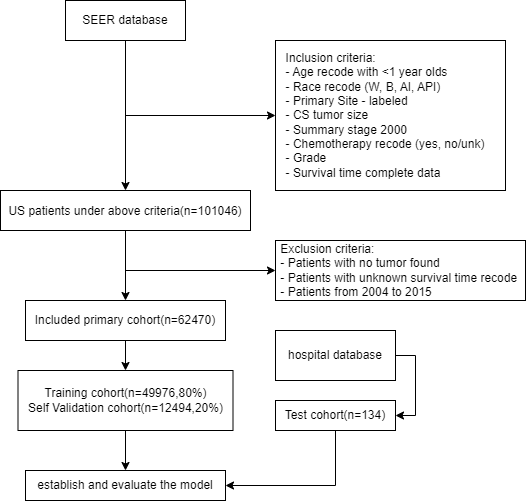
\includegraphics[scale=0.8]{paper_database.drawio.png}
    \caption{数据提取流程图} \label{fig:dataset1}
\end{figure}

由图可见,在SEER数据库中,首先提取从SEER数据库中提取数据,各字段信息将在后面的章节阐释如何筛选得到,最终得到数据101046条。然后通过排除标准,将SEERStat软件中中不能进行排除的部分不需要的数据进行脚本审查,最终分离得到需要的62470条训练用数据。将这些数据进行裁切,最后得到的是49976条训练数据与其附带的自验证数据12494条。

另一方面,由于SEER数据库中的数据存在一定局限性,其只包含被国立医学研究院认可并被SEER接收的数据。这意味着SEER的数据可能由于各地医疗情况与政策差异,不包含某些地区与特定人群的数据,如果文章使用SEER数据库进行验证,无疑会生成部分不够准确的研究内容,甚至影响将来的研究方向。因此,我从医院数据库中进行采集、梳理和标记,最后筛选得到134条验证数据,以供之后验证使用。这些数据可以验证或补充 SEER 数据,以确保研究结果的可靠性和准确性。而且从医院得到的数据也能帮助将来的研究者更好地了解特定疾病的治疗方案与效果,这些信息也会对将来的医学研究与实践具有重要的意义。

因此,使用 SEER 数据和从医院得到的数据都是重要的,以确保医学研究的结果更准确、全面和可靠。两者结合使用可以提高研究结果的可靠性和准确性,并为医学研究和实践提供更准确和有用的信息。

\subsection{SEER癌症数据库}

SEER(监测、流行病学和最终结果)计划提供大量癌症统计数据,它的目的是通过对癌症数据提供完整的监控数据,减少医疗系统中的癌症负担。SEER数据被认为是美国癌症研究的重要资源之一,因为它包括了来自不同地区的多种癌症类型的发病率和死亡率,以及提供了大量患者的年龄、性别、地理位置和治疗信息等详细信息,同时它也是国际公认的最大最成体系的癌症数据库之一。它起源于1971年美国国家癌症法(NCA)对于建立一个体系化数据库来收集、储存、分析和分发癌症相关数据,以用于支持、预防、诊断和治疗癌症的研究。SEER的病例收集从1973年1月1日开始,在美国的几个地理区间上进行诊断和提取。50年来SEER数据收集范围越来越大,同时内容也不断完整化、规范化,如今收集到的总数据已占美国人口的一半。大量来自不同种族和年龄段的癌症数据为研究者详细分析癌症提供了很大的便利。该数据集的优点是包含了多个癌症类型,且数据集中的样本数量较大,这使得研究人员可以更好地研究不同癌症类型的特点和趋势。

近年来,越来越多的研究人员开始使用该数据集来研究癌症分类和预测,每年大量有关癌症分类和预测的文章在各类期刊上发表,医学人士往往使用列线图等来提供可以在临床上进行定量使用的R语言模型,该数据集也被逐渐用于研究不同癌症类型的生物学特征和发病机制。

\subsection{医院验证数据库}

医院数据由我在医生老师们的指导下得到,如图\ref{fig:dataset_test_file}所示:

\begin{figure}[!htbp]
    \centering
    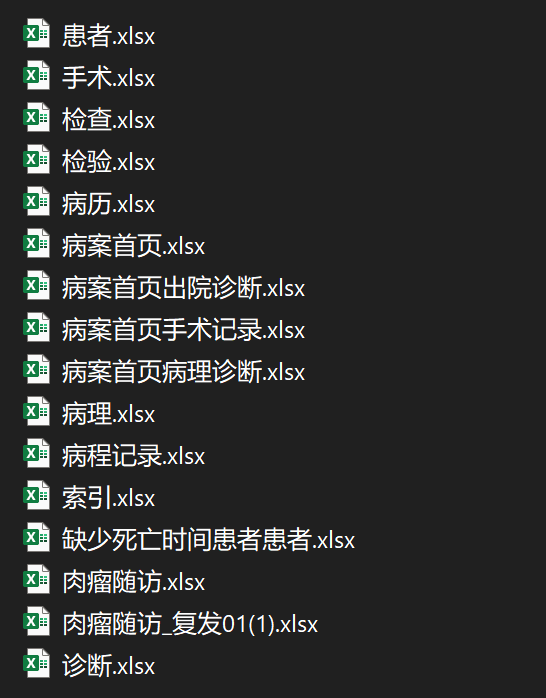
\includegraphics[scale=0.6]{hospital_dataset_files.png}
    \caption{医院原数据图} \label{fig:dataset_test_file}
\end{figure}

该数据库提供了患者的病例、检查等数据,在对其中字段内容进行遍历后,我比较了了训练数据中与验证数据中共同存在的一部分内容,并按照第\ref{cha:analyse}章分析结果确定最终纳入的变量。

\section{数据字段对应编码与含义}

从SEER数据集中,根据分析因素对生存率的相关性选择了下列字段:

\begin{figure}[!htbp]
    \centering
    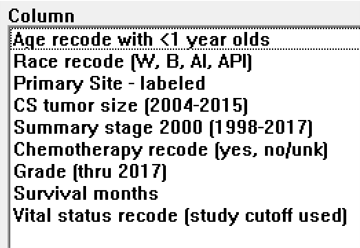
\includegraphics[scale=0.6]{seer_vals.png}
    \caption{SEERStat中选择的变量数据图} \label{fig:seer_vals}
\end{figure}

其中方括号内的时间段是由于编码方式改变产生,在不同的时间段有不同的编码方式,所以文章最终取交集2004-2015年范围间。
关于字段的解释如下:

\begin{itemize}
  \item 年龄(例:60-64 years)
  \item 种族(白人、黑人、美国印第安人/阿拉斯加原住民、亚洲人或太平洋岛民)
  \item 原发部位(子宫内膜、子宫肌层等)
  \item 肿瘤大小(最大直径)
  \item 肿瘤分期(Localized、Regional、Distant)
  \item 是否化疗(是、否/未知)
  \item 肿瘤分级(I、II、III、IV)
  \item 生存时间相关信息
\end{itemize}

文章中使用到的字段主要如上述列表所示。

首先,年龄使是以5年为一个单位所表示的,年龄重码变量是基于诊断时的年龄(单年年龄),使用的分组是由年龄决定的,年龄重新编码变量中使用的分组是由患者数据中的年龄分组决定的。这个重码变量中有19个年龄组(\textless1岁,1-4岁,5-9岁,...,85岁以上)。

第二个字段是种族,在SEER数据库中,主要有六个选项,他们分别是白种人、黑种人、美国印第安人/阿拉斯加原住民、亚洲人或太平洋岛民、其他未说明的(1991年以上)。考虑到在测试数据集中,我们使用的是中国人作为主要的测试患者,一开始我只使用了亚洲人或太平洋岛民的数据,但是在之后的模型建立中,我发现如果只使用亚洲人和太平洋岛民作为训练数据的话模型的效果并不好。可能的原因是亚洲人和太平洋岛民中存在着显出的差异,另一种可能的解释是数据量的不足。考虑到该字段频数的差异我最后使用了白种人黑种人和亚洲人或太平洋岛民作为训练集中开始算的参数选项。

文章使用的第三个字段是原发部位(Primary Site),这个字段主要表示病发的部位。这个字段提供了ICD-O-3规范的主要部位代码和一个描述性的主要部位标签该标签是首选的ICD-O-3加粗的名称,其他部位或子部位包含在代码中,但没有反映在代码中,本文使用的子宫肉瘤数据都包含ICD-O-3标签。编码中可能还包括其他部位或子部位,但没有反映在首选标签中。诊断年份在1992年之前的病例从早期版本转换为了ICD-O-3。这里亦只选取了四个选项,见图\ref{fig:seer_exclusion}中。

第四个字段是肿瘤大小,肿瘤大小指的是肉眼所见肿瘤的最大直径。肿瘤大小适用于2004-2015年的诊断年份。早期的病例部分会被转换,并增加新的编码以加以匹配,这些编码在目前的CS版本之前是不可用的,而且在当前版本的CS之前无法使用的新编码。关于肿瘤大小的详细说明见图\ref{fig:tumor_size}。

\begin{figure}[!htbp]
    \centering
    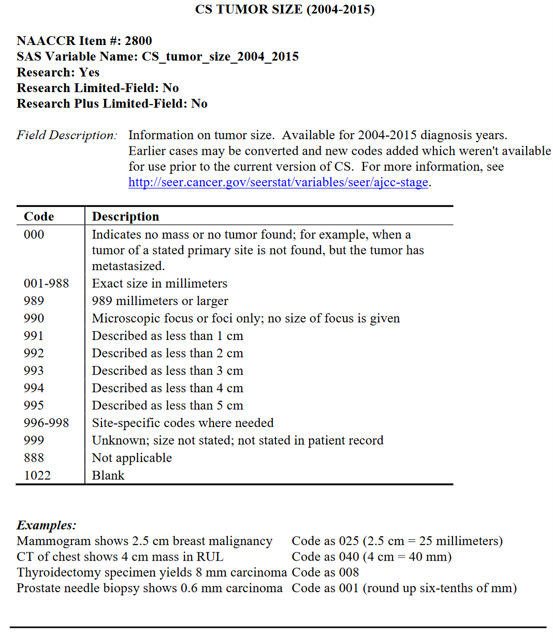
\includegraphics[scale=0.4]{tumor_size.png}
    \caption{SEER数据库中CS Tumor Size字段的详细说明图} \label{fig:tumor_size}
\end{figure}

肿瘤分期是指对恶性肿瘤进行分期分类的过程,它用于描述肿瘤的扩散程度和位置等特征,以便更好地评估肿瘤的严重程度和治疗前景。肿瘤分期通常由国际癌症联合会制定,其分期系统根据不同的肿瘤类型和特定癌症的组织学和生物学特征而有所不同。SEER主要使用的是TNM分期系统。TNM是一个在国际中广泛应用的为肿瘤进行而实现的系统,在它的分类标准中,主要针对以下几个方面进行分期:肿瘤的大小、淋巴的侵扰情况、肿瘤的转移与否。这里使用的是M标准,肿瘤的转移与否,主要分为三种情况,分别表示局部区域与远端三种类型。其中局部表示肿瘤仅限于原始的发生位置,没有扩散到周围组织或器官。区域表示肿瘤扩散到周围组织或病变器官,但没有扩散到远处的器官或淋巴结。远端则表示肿瘤已经扩散到其他远隔的器官或淋巴结。肿瘤分期表示了肿瘤扩散的进展过程,是对患者生存率有较大影响的一个影响因子。

化疗与否标识了患者是否使用了化疗作为辅助治疗手段。这里要主要的一点是由于患者隐私和机构编码原因,使用的两个编码分别是“是”和“否/未知”,这样的编码会对准确率产生一定的影响。

肿瘤分级是指对恶性肿瘤进行分期的的一种方法,它可以根据肿瘤的大小、形状、密度和边缘等特征来评估肿瘤的恶性程度。肿瘤分级通常由医生进行视觉评估,也可以通过计算机辅助断层扫描(CT)、磁共振成像(MRI)和其他影像学技术来进行辅助评估。这里一个分为四个等级:

\begin{itemize}
\item 等级一:这个等级是最低的,在这个等级中,肿瘤的分化情况最低,肿瘤细胞构成的组织和正常工作的组织差别较小,这种情况也常常被书面称为分化良好,肿瘤的恶性化程度最低。
\item 等级二:在这个等级中,肿瘤细胞已经开始出现一定的明显不同,这不但体现在肿瘤细胞的生长周期已经与正常细胞有明显的差异,而且肿瘤的形态也与其他组织有不同,这类组织恶性程度已经较高。
\item 等级三:这类肿瘤组织等级被称为分化最差的,这意味肿瘤的分化程度较差,大部分肿瘤细胞已经没有正常组织的功能表现了,内部是大量无定形的而无法描述的细胞,这类细胞由于分化程度低,所以增殖速度也最快,不成组织的细胞也最易向周围组织侵扰,所以危险程度也最高。
\item 等级四:这个等级表示未分化,这意味着肿瘤的分化程度最低,其中几乎没有分化的细胞,在临床中出现极少。
\end{itemize}

以上数据中,肿瘤大小、肿瘤分期、肿瘤分级与生存相关内容外的数据都可以直接使用SQL语句或Python脚本简单提取,这里我使用了ipynb文件作为提取方案,以适应研究过程中的大量更改。生存相关数据在数据库中并没有记录,所以我使用脚本筛选了所有提供联系方式的患者的信息,在医院方面进行随访后对得到的数据进行提取。

而肿瘤大小、肿瘤分期与分级数据没有直接字段提供,只能从病理分析中的诊断文本中提取,我首先筛选了其他字段记录完整的患者,并在这些数据的诊断信息中提取。肿瘤大小这里选取的是左附件区和右附件区中的最大肿瘤的最大直径,所以我编写了相应的Python 简单NLP算法,文本的左附件右附件的划分,并在这两段中分别找到用以描述肿瘤的大小。由于还有关于回声区和输卵管长度等的干扰,必须严格找到肿瘤对应的大小。最后在得到的所有肿瘤大小中找到最大值并返回。无匹配内容的描述只能得到空值作为回应,所以最后我对所有数据进行了人工校验。而肿瘤分期与分级同理,先在文本中检索是否有直接指明的描述,如果没有则按照上文中的定义来确定相应的内容。

通过上述的处理,初步筛选得到的300条数据在去除上述内容的缺失后一共是134条测试数据。

\begin{figure}[!htbp]
    \centering
    
\includegraphics[scale=0.4]{seer_exclusion.png}
    \caption{SEERStat中选择的变量排除条件图} \label{fig:seer_exclusion}
\end{figure}

% !Mode:: "TeX:UTF-8"
\chapter{可行性分析与生存分析}
\label{cha:analyse}

\section{可行性分析}

\subsection{技术可行性}

通常对于生存分析与建立预后模型使用的是R语言,然后考虑到后期需要将训练得到的模型与后端进行组合,而且R语言的使用人数较少,没有完整的社区资源可供查询,而且为了减少最终系统的复杂度,最后使用了Python作为主要框架的语言。而Python中虽然官方包并没有支持生存分析与模型建立的内容,但是Python有大量第三方包可供调用。在Python中,可以使用的生存分析包的数量没有限制,只要这些包相互兼容,不造成冲突。如lifelines、scikit-survival、survival、pysurvival和scipy。每个包都有自己的优势和劣势,包的选择取决于分析的具体需要和目标。lifelines具有易于使用的API,用于常见的生存分析任务,如Kaplan-Meier估计、Cox比例危害回归和加速失败时间模型。支持随时间变化的协变量、左截断和区间删减。提供可视化工具,如生存曲线、危险函数和累积危险函数。虽然它对灵活的参数化生存模型和对竞争性风险分析的支持有限。但是在目前的标准下其已足够完成分析任务。而相比于lifelines,其他包比如scikit-survival相对于图形化的支持不足,而pysurvival由于复杂的语法和有限的文档,学习曲线可能很陡峭,scipy则ui较为简陋。所以最后选择了lifelines作为主要分析工具。

在后端方面,相比于Java的SpringBoot框架,Flask的环境要求相对较小,也比较容易编写相应的Dockerfile以满足简单的部署。同时考虑到和使用Python的模型结合,如果使用相同语言则可以直接将模型嵌入其中,所以最后使用了Flask作为主要框架。而笔者在大学期间与实习过程中已经积累了相应的在服务器、开发板中部署环境的经历。考虑到经济价格原因,最后的Flask项目先后在阿里云与树莓派开发板上完成过部署,已经确认Flask端的程序具有良好的部署性能与健壮性。而且Flask的良好接口文档也让这项工作有更多的资料可以参考学习。

在前端方面,本文使用的是Vue3作为框架,这里使用的是组合式API开发,相比于Vue2延续而来的选项式API,Vue3的结构更加清晰,使用了少缩进的组合展开方式,可以直接在setup中使用ref、watch等函数来分别管理变量和监控生命周期。这也为开发和后期更改提供了便利。

综上所述,通过分析患者生存情况训练预后模型,并开发使用Vue3-Flask的的管理系统具有技术可行性。

\subsection{其他可行性}

本系统成本主要包括软件开发成本、版权使用成本、硬件维护成本、数据收集成本。其中软件开发完全由笔者承担,除了占用的时间资源外不消耗其他费用。UI界面中使用的主要是Element-ui提供的图表等资源,MIT协议起源于麻省理工学院,是在所有软件许可中比较宽松的一种,授权人或使用者具有完全的使用、复制、更改、分发等等权力,所以使用相应的资源并不会消耗版权成本。硬件分别使用了阿里云和树莓派用来测试部署效果,阿里云仅仅使用了一个月,成本为12元,而树莓派在之前就已获取,在家运行成本忽略不计。数据来源分别来自SEER数据库与本地医院,SEER数据集中的数据较为完整,笔者通过提交申请后得到授权,随即即可访问相应软件并通过提取得到;而医院数据由于有关患者隐私具体细节不能公开,主要由数据库中进行笔者进行提取,而医院方面配合进行随访,最后由笔者与医院方面共同标记数据得到最后的测试数据。

综上所述,本文进行开发的资源和内容明确,经济成本在可负担范围内,同时使用的材料和内容都不侵犯相关法律条例或其他团体或个人权益,同时时间成本和开发技术栈都进行了有效的权衡,因此该项目可行性得证。

\section{需求分析}

\subsection{目标对象分析}

预后模型的主要面向对象是术后的子宫肉瘤患者和相关专业的医生与管理者,考虑到为了避免可能存在的恐慌和信息泄露,该模型及相关系统不会直接向患者或者大众开放,而是用于医疗数字化的应用,比如在医院内网或其他方面搭建。而考虑到使用对象是来自医院的医生、管理员以及后期维护人员,所以一个清晰的UI界面和所见即所得的管理面板是需要的,同时主要的两个用户角色也需要配备相应的权限管理与账户管理。同时为了方便管理员或后台维护人员进行后期的内容增广与技术更新,系统内部同样要配备一定的工单或消息处理与记录功能。从而能让各个角色都能迅捷而高效的完成各自所需要完成的工作。

另外,考虑到数据收集过程到最后模型中预测的不同,同时由于JS到Flask中的表单信息和数据格式需要进行的变化。从前端到后端需要设计一个映射从而不影响数据的准确使用和训练。

\subsection{功能需求}

考虑到医院、医生多方面的需求,以及患者的实际需求,预后模型有以下几个功能或特点选项:
\begin{enumerate}
    \item 对于患者的预后数据,模型需要能够输入规定的所有患者数据,包括患者的年龄、肿瘤大小等,并根据这些数据进行推断
    \item 预后模型的输出要求可以有多种,比较常用的做法是单单对患者的三年或五年生存率进行判断,如果模型具有概率层,一个概率也将是可以选择的输出,可以用来描述该结果的准确度,以供医生了解结果的准确度。而在后文中,笔者将介绍一种新的方法,使用聚类来将患者分群,此时预后模型的输入相同,而输出则是患者的表征群。这个方法看似只评估了聚类的结果,结果没有之前的有意义。然而,实际上这个结果更加有统计学意义,因为相近的病情状况往往意味着病情的危险程度相近,所以这个结果也具有更好地判断有效性,对于临床使用的可行性也更好。
    \item 模型需要分析出各个输入因素的重要性,从而令模型有更好的解释性,对于树型模型需要有图显示其结构。
\end{enumerate}

而一体化平台则需要具有以下几个功能:
\begin{enumerate}
    \item 一个登录界面,用来进行基础的账号管理,登录时需要提供用户名与密码。后台存储的账号分别分为管理员与普通医生,需要hash加密密码以让用户登录更加安全,管理员具有访问更高级别页面的权限。考虑到信息安全问题不提供直接使用token或其他第三方机构账号登录。
    \item 系统首页,首页可以显示用户的头像和登录位置等信息,同时也显示当前用户上传的数据量与预测患者人数,通过对该功能的增广可以让管理员更方便地布置任务,显示其他信息等。
    \item 数据表格页面,数据表格可以显示按照上述规范的带标注的详细数据信息,数据实际信息在后台通过端口处理将接收到的文件按照映射表转换为csv格式的编码信息。这样的操作可以明显减少数据文件的体积,减少占用的内存。同时,数据表格页面同时提供了表单功能,从而方便医生录入新的数据并校验数据正确性。
    \item 工单记录功能,有关系统本身和待处理的信息都会在这个页面显示,符合权限要求或指定的接收用户能够在这个页面看到这个信息,而如果信息已经被读取则会标为已读。同时还提供了回收站功能来防止用户误删信息。
    \item 训练模型页面,训练模型页面提供了直接上传数据文件的功能,上传数据文件后,文件将通过js判断基础格式是否符合要求,如果符合就会被上传到后端中进行模型训练,训练完成后模型文件将会暂存在后端中,同时该页面下的数据表格也会显示当前的模型名称和评分等信息。如果选择不保存或删除模型,后端将会同时删除使用的表和模型文件。
    \item 预测数据页面同样提供了表格用来存储历史数据。用户可以选择使用的模型并通过直接填写页面中的表单并点击预测键即可预测患者的状况,为了方便起见,这里只选取了患者三年死亡与否的结果预后模型。在这里患者的详细信息被隐去,取而代之的是患者的三年生存与否和当前结果准确率的数据。这些历史记录同样有删除功能
    \item 权限管理页面,权限管理页面提供了上述各页面的权限更改功能。其中只有管理员可以修改用户角色,而也只有管理员可以添加新的角色并赋予给用户。管理员可以给用户角色设置对每个页面能否访问。
\end{enumerate}

\section{变量选择}

在研究过程中,笔者首先阅读了一些有关子宫肉瘤列线图与模型相关的文章\cite{novel_tool},在这些文章中,年龄、种族、地区、婚姻状况、肿瘤大小、淋巴结状态、分期、分级、化疗、放疗都是比较常用的数据。然后在对SEER的数据集进行筛选后,我发现主要的库中婚姻状况等参数由于隐私原因被移除,而淋巴结的信息符合标准的过少,如果使用则会大大削减符合要求的数据数量,从而让训练集变得很小,所以考虑到这点后没有纳入。与医院老师们沟通后,笔者发现分期中的一些描述包含了淋巴结是否被侵犯的状况,而目前医院内主要使用化疗作为主要手段,放疗的数据较少所以没有考虑纳入,所以最后选择了选择了当前的变量。

\section{生存分析}

\subsection{数据概况}

从SEER数据集中采集到的数据一共有62470条,患者的年龄分布如下图所示:
\begin{figure}[!htbp]
    \centering
    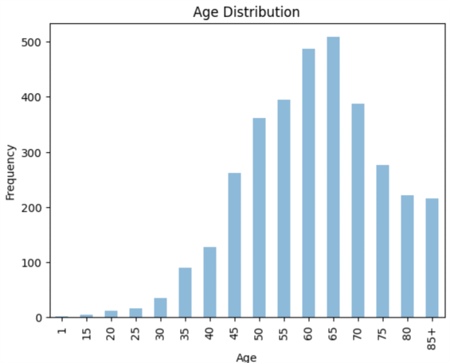
\includegraphics[scale=0.8]{age_distribution.png}
    \caption{SEER数据集中患者年龄分布图} \label{fig:age_distribution}
\end{figure}

由于基数较大,同时表格中的数值取区间中的最低值,表中的频数对其进行了平均缩减以方便显示,可以看到表格中用户的年龄主要集中在60-70之间,这说明了患者的年龄越大,越有可能患子宫肉瘤,如果按照三分位数进行划分,我们可以得到子宫肉瘤的主要发病人群集中在45岁到65岁之间。

而对于另外一个数值变量,肿瘤大小的分布如下图所示:

\begin{figure}[!htbp]
    \centering
    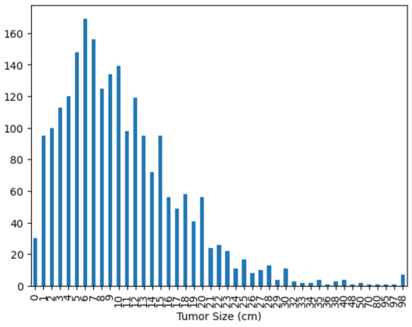
\includegraphics[scale=0.8]{tumor_size_distribution.png}
    \caption{SEER数据集中患者肿瘤大小分布图} \label{fig:tumor_size_distribution}
\end{figure}

按照上述表格同样可以得到肿瘤大小的大致分布,在表格中可以看到,肿瘤大小的中间值在50mm左右,肿瘤大小为0mm代表1mm以下或较难以衡量的数据,而肿瘤大小在到达50mm的峰值后则呈反曲线状态减少,直到到达最低点。肿瘤大小的分布较为复杂,因为这个原因所以我们也很难为其划分一个清晰的界限来划分患者,如果直接划分很可能会损失一部分信息。这里先使用50mm为分界点进行划分,后期再是用其他方法进行比较。

\subsection{Kaplan-Meier曲线绘制}

由于下面使用的Cox比例风险模型需要数据满足以下假设:
\begin{enumerate}
    \item 风险比值的对数与协变量之间呈线性关系
    \item 风险比值的对数与时间无关
\end{enumerate}

上面的风险比值的对数与协变量之间呈线性关系假设需要使用Kaplan-Meier曲线进行验证。具体方法是:对于同一自变量,如果本身为分类型变量直接使用,如果为连续或数值型变量,则把变量分为多个区间作为不同值,观察曲线间状态,如果曲线存在交叉则说明其不满足假设,反之则说明风险比值和协变量间存在线性关系,满足条件。

同时,KM曲线不但可以验证后续的假设是否成立,同时也能对患者的生存状况做更细致的分析。KM曲线的原理是首先计算在某一时期存活的病人能活到下一时期的概率,然后将存活概率逐一相乘,得到相应时期的存活率。这种方法可以非常清晰地看到两组患者在不同时间的生存率差异。

由于篇幅问题,这里仅列举两张比较典型的进行分析说明:

\begin{figure}[!htbp]
    \centering
    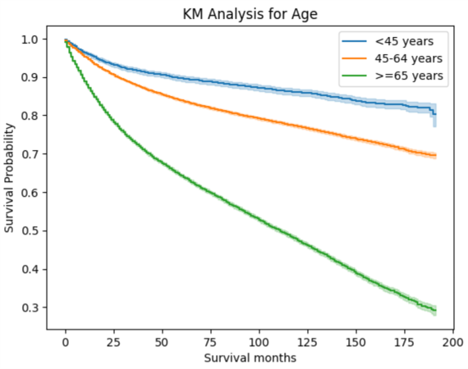
\includegraphics[scale=0.8]{km_age.png}
    \caption{SEER数据集中患者年龄KM曲线图} \label{fig:km_age}
\end{figure}

从图\ref{fig:km_age}中可以看到,45岁以下的患者在时间变化下衰减最少,而45-64的次之,65以上减少最快,而这些曲线都不交叉,置信区间也较小。这说明了患者的年龄是一个重要影响因素,而患者的年龄越小,生存率越高。

\begin{figure}[!htbp]
    \centering
    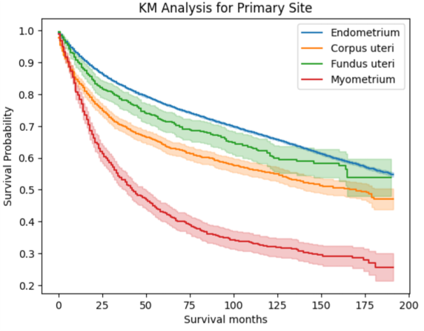
\includegraphics[scale=0.8]{km_site.png}
    \caption{SEER数据集中患者原发部位KM曲线图} \label{fig:km_site}
\end{figure}

从图\ref{fig:km_site}中可以看到,四个原发部位的患者生存率从高到低的变化,从置信区间的的范围可以看到四者的数据量也存在差异。同时这些组间也存在线性比例关系,所以满足假设。

\subsection{Cox单因素分析}

Cox单因素分析是一种基于Cox比例风险模型的统计分析方法,它可以用于研究变量对于结果的影响。本文使用年龄、种族、原发部位、肿瘤大小、分期、化疗情况、分级建立Cox模型,并使用SEER数据集中的数据编码为合适格式,用编码后的结果训练。下列的表\ref{tab:cox_univar}是单因素模型的Cox分析结果。

\begin{table}[htb]
    \centering
    \begin{minipage}[t]{0.8\linewidth} 
    \caption[预测子宫肉瘤患者总生存率的单变量Cox分析]{预测子宫肉瘤患者总生存率的单变量Cox分析}
    \label{tab:cox_univar}
      \begin{tabularx}{\linewidth}{lXX}
        \toprule[1.5pt]
        {\heiti variable} & {\heiti exp(coef)} & {\heiti P value} \\\midrule[1pt]
        \textbf{Age} \\
        \textless45years \\
        45-64years & 1.68 & \textless0.005 \\
        $ \geq $65years & 4.35 & \textless0.005 \\\midrule[1pt]
        \textbf{Race} \\
        White \\
        Black & 0.56 & \textless0.005 \\
        Asian or Pacific Islander & 0.47 & \textless0.005 \\\midrule[1pt]
        \textbf{Primary Site} \\
        C54.1-Endometrium \\
        C54.9-Corpus uteri & 1.67 & \textless0.005 \\
        C54.3-Fundus uteri & 1.43 & \textless0.005 \\
        C54.2-Myometrium & 3.24 & \textless0.005 \\\midrule[1pt]
        \textbf{Tumor Size} \\
        \textless50mm \\
        $ \geq $50mm & 2.36 & \textless0.005 \\\midrule[1pt]
        \textbf{Stage} \\
        Localized \\
        Regional & 2.72 & \textless0.005 \\
        Distant & 10.94 & \textless0.005 \\\midrule[1pt]
        \textbf{Chemotherapy} \\
        Yes \\
        No/Unknown & 0.41 & \textless0.005 \\\midrule[1pt]
        \textbf{Grade} \\
        Well differentiated; Grade I \\
        Moderately differentiated; Grade II & 1.84 & \textless0.005 \\
        Poorly differentiated; Grade III & 4.93 & \textless0.005 \\
        Undifferentiated; anaplastic; Grade IV & 6.95 & \textless0.005 \\
        \bottomrule[1.5pt]
      \end{tabularx}
    \end{minipage}
  \end{table}

coef是Cox中的回归系数beta,因此exp(coef)是Cox比例风险模型中的概率风险比。从结果中可以看到,计算得到的P值是用来评估同一变量的协变量对因变量的影响是否显著的参数。这里使用变量中的第一个协变量作为参照,分析其他协变量是与对照变量存在显著差异。一般在0.05以下则说明变量对于结果的影响较为显著,可以看到表中的结果都在该值之下,所以说明每个变量的不同值对于计算结果的影响较为显著,同时也验证了在Kaplan-Meier曲线中观察到的结果。

\subsection{Cox多因素分析}

Cox多因素分析也是一种基于Cox比例风险模型的统计分析方法,它可以用于研究多个不同的变量对于结果的影响。下列模型同样使用年龄、种族、原发部位、肿瘤大小、分期、化疗情况、分级建立Cox模型,并使用SEER数据集中的数据编码为合适格式,用编码后的结果训练。不同的是单因素将变量的每个值作为参数导入,而且同时只导入一个变量,而多因素分析则直接导入有不同值e多个变量。下列的表\ref{tab:cox_multivar}是多因素模型的Cox分析结果。

\begin{table}[htb]
    \centering
    \begin{minipage}[t]{0.8\linewidth} 
    \caption[预测子宫肉瘤患者总生存率的多变量Cox分析]{预测子宫肉瘤患者总生存率的多变量Cox分析}
    \label{tab:cox_multivar}
      \begin{tabularx}{\linewidth}{lXX}
        \toprule[1.5pt]
        {\heiti variable} & {\heiti exp(coef)} & {\heiti P value} \\\midrule[1pt]
        \textbf{Age} & 2.23 & \textless0.005 \\
        \textbf{Race} & 0.82 & \textless0.005 \\
        \textbf{Primary Site} & 1.17 & \textless0.005 \\
        \textbf{Tumor Size} & 1.52 & \textless0.005 \\
        \textbf{Stage} & 2.47 & \textless0.005 \\
        \textbf{Chemotherapy} & 1.29 & \textless0.005 \\
        \textbf{Grade} & 1.56 & \textless0.005 \\
        \bottomrule[1.5pt]
      \end{tabularx}
    \end{minipage}
  \end{table}

从结果中可以看到,计算得到的P值是用来评估多个变量对因变量的影响是否显著的参数。这里由于不是同一变量,所以不需要像单变量分析一样使用变量中的第一个协变量作为参照,分析其他协变量是与对照变量存在显著差异,相反,由于多个变量互不交叉,其是并不需要设置一个变量作为参照组。一般在0.05以下则说明变量对于结果的影响较为显著,可以看到表中的结果都在该值之下,所以说明每个变量对于计算结果的影响较为显著。这是在Kaplan-Meier曲线阶段无法观察到的多变量影响,这说明不但单个变量的不同值对于结果有比较大的影响,同时这个结果也可以在多变量模型中观察到,进一步验证了所选取的变量都有纳入价值。

\subsection{生存分析结论}

在上述对于患者数据库内数据分布的分析后,本文分别进行了Kaplan-Meier曲线的绘制和Cox单变量和多变量分析。其中对于数据的分布分析让我们对于数据库中的人群特征有了一定的了解,同时也为如何对变量类型为数值变量的变量进行了一定的划分,从而方便后续在Cox模型中导入并训练。而Kaplan-Meier曲线的绘制有两个目的,第一个目的是可以初步对于不同变量对结果的影响,从而让我们能够初步对于是否纳入该变量有一定的预判,在之前的工作中,笔者对于如何纳入变量有了较多考量,其中首先从论文中选择了一些常用的、对结果影响较大的变量,同时也选择了一些其他的未纳入过的变量,而这些变量中的一部分便因为KM曲线结果不符合模型标准或在这之前便发现变量内容与其他变量具有重复或冲突,所以最后没有纳入。而如果在这个阶段提前使用Kaplan-Meier曲线进行分析的话可能就能避免之前的重复劳动。Cox单因素模型分析选择了每个变量的不同值,将它们进行了拆分为二元变量并堆叠为组的过程,从而导入Cox单因素模型进行分析,在这个过程中,可以得到之前使用Kaplan-Meier曲线不能看到的的精确数值表示,这样便可以让我们对于数据是否能够纳入得到一个更明确地标准,而不是对于曲线进行经验判断。而多因素分析则解构了多个变量,分期它们结合起来对于结果的影响是否显著,这里与之前不同,如果只有单个变量只需要使用 log-rank 检验来确定因素之间的显著性关系即可,而多变量则需要使用比例风险回归模型才能确认影响,如果某一变量在 log-rank 检验中显示影响较大,在多变量回归中可能会因为其他变量占比较大从而反而显示不出较好的影响。而当前结果表明,目前采用的变量都对于结果有较为显著的影响,在之后的模型纳入与训练中可以作为参数使用。

% 致谢
\begin{acknowledgement}
  衷心感谢导师 沈文枫 教授对本人的精心指导。
  同时感谢同济医院 袁素珍老师、汪雯雯老师 对工作的支持和
  上海大学开源社区提供的 \LaTeX 模板。
\end{acknowledgement}


\bibliographystyle{shuthesis}
\bibliography{reference/refs}

\backmatter
\begin{appendix}
\chapter{经典不等式}
论文中用到的经典不等式.\\

\noindent{\bfseries (H\"older Inequality)}
设~$a_i\geq0$, $b_i\geq0$, $i=1$, $2$, $\cdots$, $n$, 且~$p>1$, $q>1$ 
满足~$1/p+1/q=1$. 则有
\[
\sum_{i=1}^{n}a_ib_i\leq\left(\sum_{i=1}^{n}a_i^p\right)^{\frac1p}
\cdot\left(\sum_{i=1}^{n}b_i^q\right)^{\frac1q},
\]
等号成立当且仅当存在一个常数~$c$ 满足~$a_i^p=cb_i^q$.\\

\noindent{\bfseries (PM Inequality)}
设~$x_1$, $x_2$, $\ldots$, $x_n$ 是~$n$ 个非负实数. 如果~$0<p<q$, 那么
\[
\left(\frac{x_1^p+x_2^p+\cdots+x_n^p}{n}\right)^{\frac{1}{p}}\leq
\left(\frac{x_1^q+x_2^q+\cdots+x_n^q}{n}\right)^{\frac{1}{q}},
\]
等号成立当且仅当~$x_1=x_2=\cdots =x_n$.\\

\noindent{\bfseries (AM-GM Inequality)}
设~$x_1$, $x_2$, $\ldots$, $x_n$ 是~$n$ 个非负实数. 则有
\[
\frac{x_1+x_2+\cdots+x_n}{n}\geq\sqrt[n]{x_1x_2\cdots x_n},
\]
等号成立当且仅当~$x_1=x_2=\cdots =x_n$.
\end{appendix}

\end{document}
